\section{ \ac{BLE} beacons}
\label{sec:beacon}


The beacons that were utilised are Texas Instruments CC2650STK devices which can be visualised in figure ~\ref{fig:beacon}. Alongside the device, which comes with a pre-installed bluetooth low energy program capable of giving information on each of its ten sensors through its predefined profiles, there is a texas smartphone application that can connect to a single device and read from its sensors. By using the texas Code Composer Studio (CSS), the pre-defined \ac{BLE} profile existent on the device could be altered.
The initial idea was to insert a new service into the already existing profile making use of the generic files provided by Texas. 
In order to implement the service, a characteristic containing the device's server IP and port was created and two random 128-bit UUID were generated. When using UUIDs, the Bluetooth SIG defined several UUID, each associated with a certain service, such as heart rate or glucose services \cite{bleservices}. This situation makes it so that whenever someone intents to implements a new service he has to generate a random 128-bit UUID for his service and another one for each of required characteristics.
Despite the efforts made, it wasn't possible to alter the existent profile by adding the new service neither by simply attempting to alter it by removing existent services. Due to the low amount of existent information on the technology an alternative was created. The solution found was to store the information into an already functioning service's characteristics as one was capable of altering those kind of parameters. The characteristics available to be used were only the ones from the device information service, a service defined by the bluetooth sig, since the remaining services on the \ac{BLE} device were meant for reading values of from sensors. The chosen characteristic was the Manufacturer's name due to its relevance and the fact that its UUID was known, while the remaining's weren't.


\begin{figure}
	\centering
		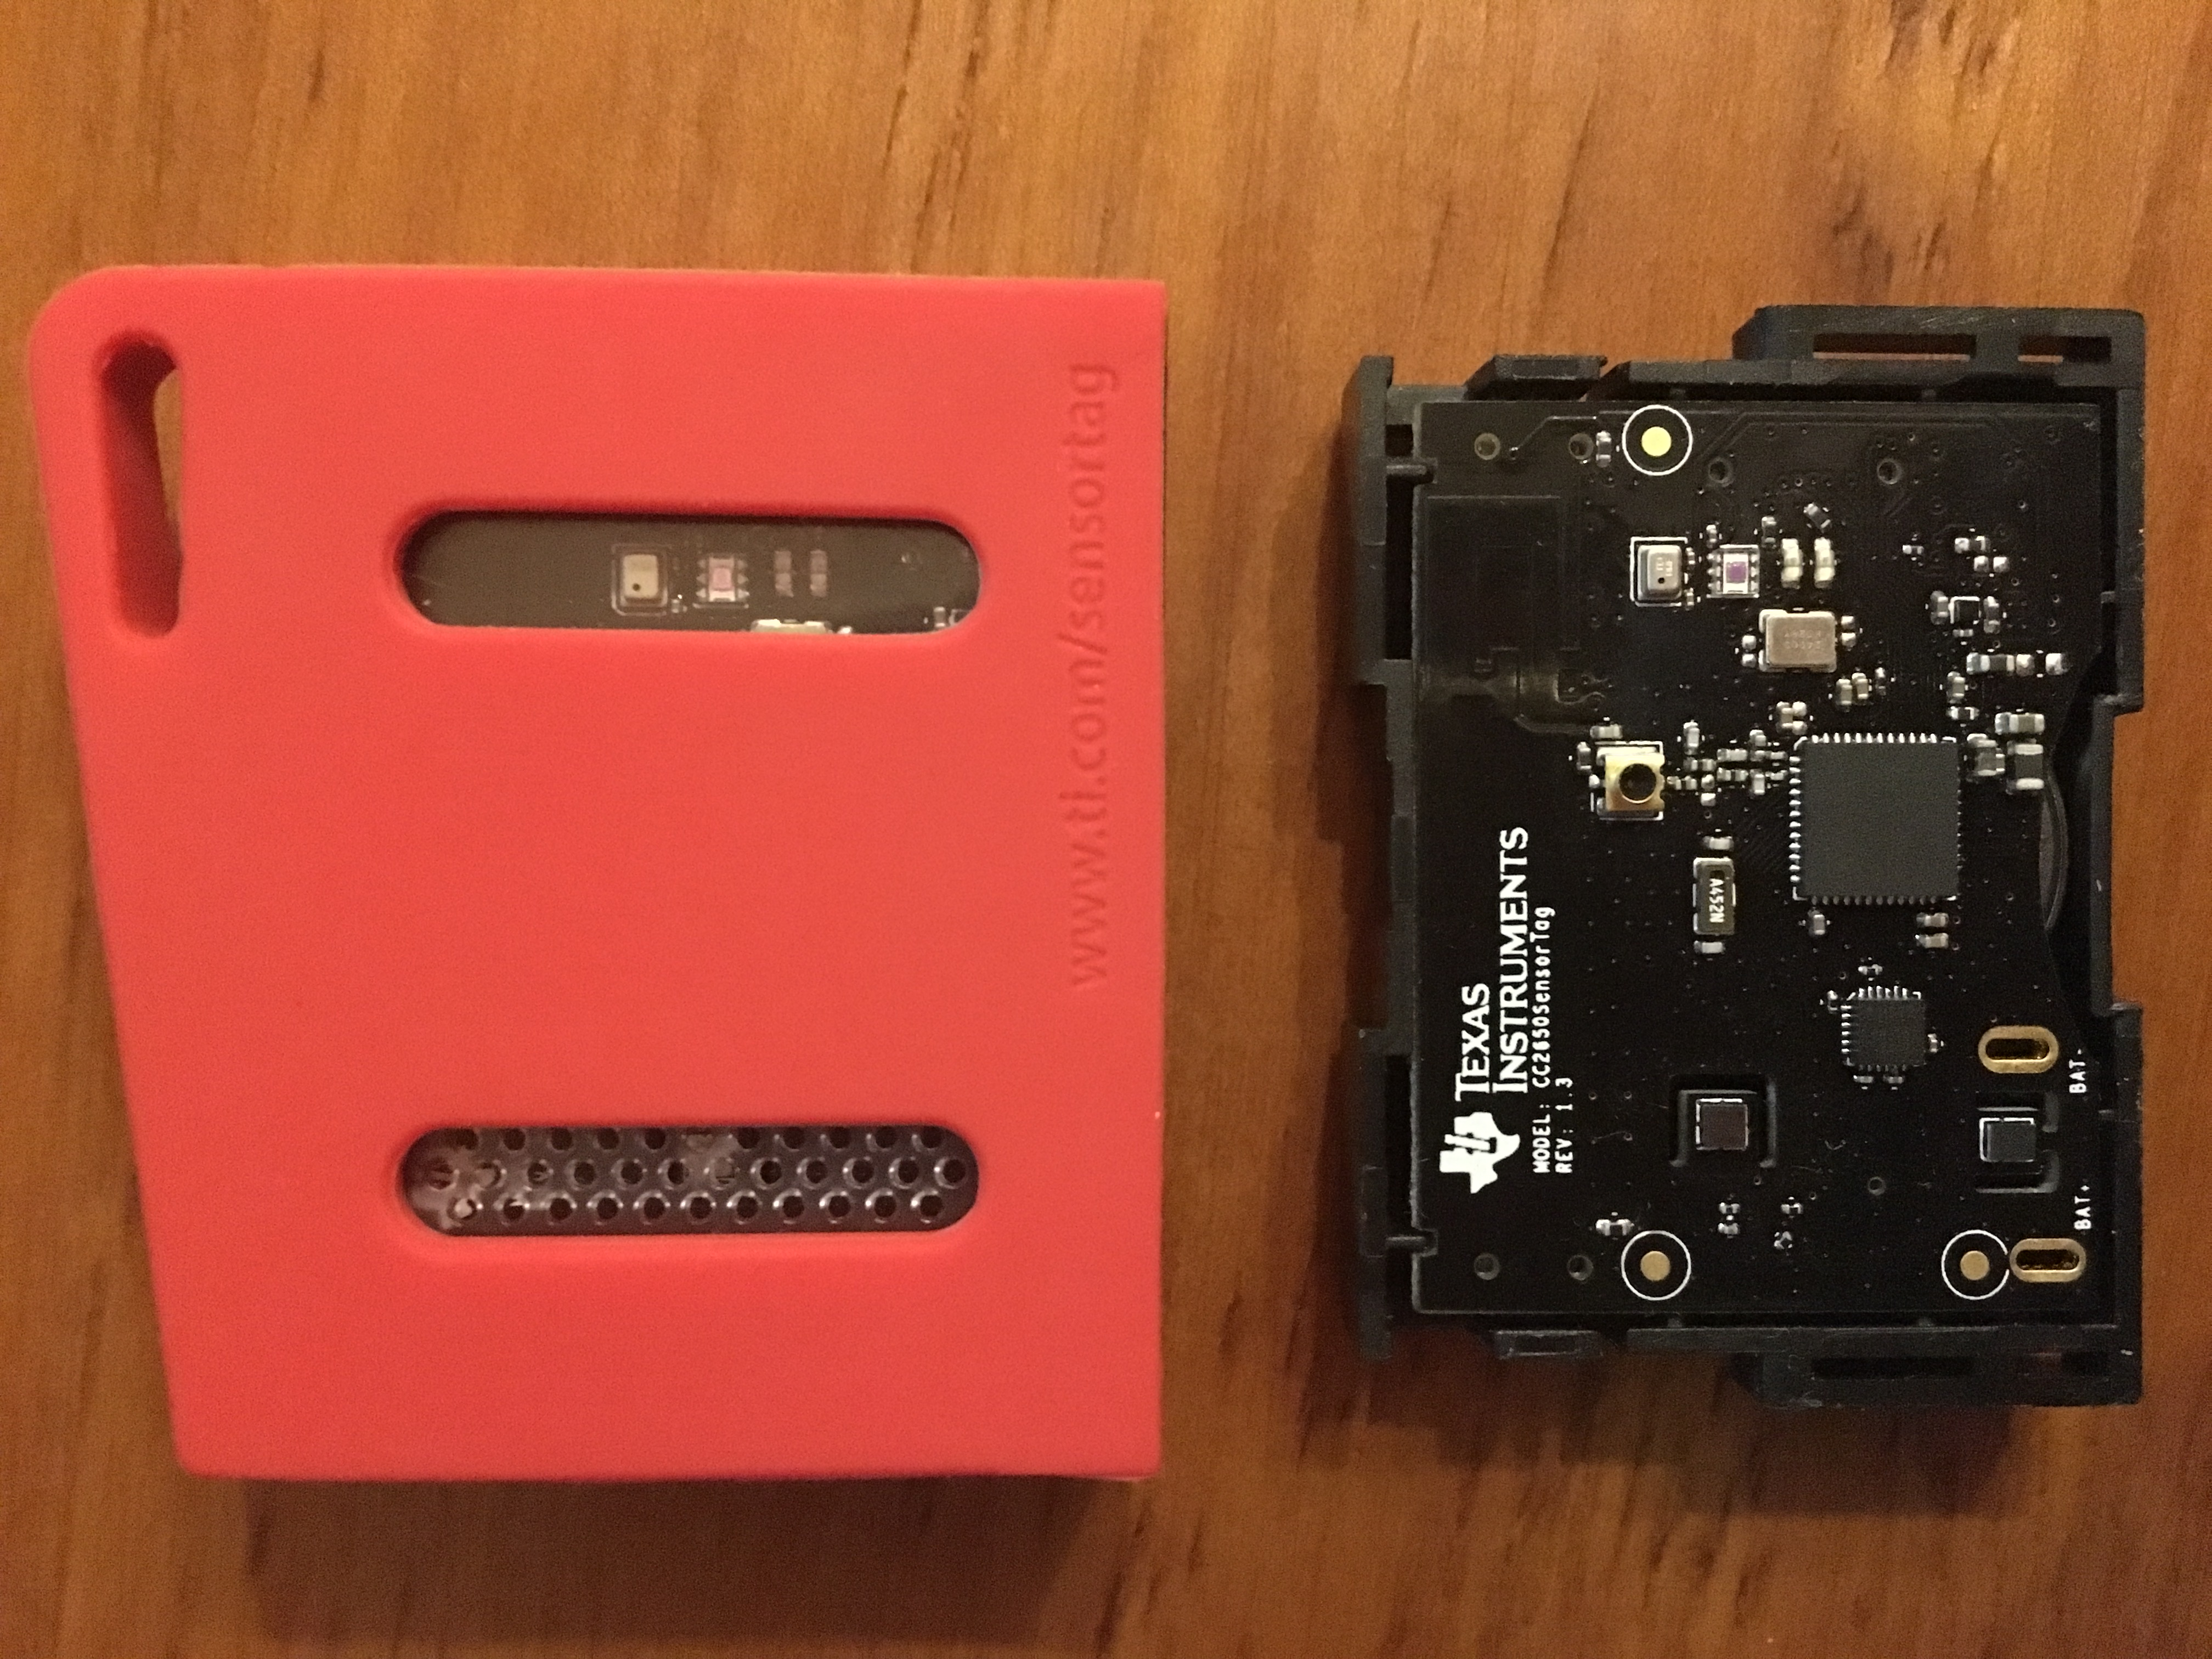
\includegraphics[width=0.5\linewidth]{4.Chapter/beacon.jpg}
	\caption[TI cc2650stk sensortag]{TI cc2650stk sensortag}
	\label{fig:beacon}
\end{figure}
